\documentclass[a4paper]{article}

%% Language and font encodings
\usepackage[english]{babel}
\usepackage[utf8x]{inputenc}
\usepackage[T1]{fontenc}

%% Sets page size and margins
\usepackage[a4paper,top=3cm,bottom=2.2cm,left=2.7cm,right=2.7cm,marginparwidth=1.75cm]{geometry}

%% Useful packages
\usepackage{amsmath}
\usepackage{amsfonts}
\usepackage{bm}
\usepackage{graphicx}
\usepackage[colorinlistoftodos]{todonotes}
\usepackage[colorlinks=true, all colors=blue]{hyperref} %referenze linkate
\usepackage{booktabs}
\usepackage{siunitx}  %notaz. espon. con \num{} e unità di misura in SI con \si{}
\usepackage{xcolor}
\usepackage{colortbl}
\usepackage{bm}
\usepackage{caption} 
\usepackage{indentfirst}
\usepackage{physics} 
\usepackage{rotating}
\usepackage{tabularx}
\usepackage{url}
\usepackage{pst-plot}
\usepackage{comment} %per usare l'ambiente {comment}
\usepackage{float} 
\usepackage{subfig}
\usepackage[americanvoltages]{circuitikz} %per disegnare circuiti
\usepackage{tikz}
\usepackage{mathtools} %per allineare su più linee in ambiente {align} o {align*}
\usepackage{cancel}
\usepackage{listings}
\renewcommand{\CancelColor}{\color{lightgray}}
%\setlength{\parindent}{0cm}


%%%%%%%%%% HEADERS AND FOOTERS %%%%%%%%%%%%
\newcommand{\theexercise}{Ex. 5}
\newcommand{\thedate}{November 9, 2020}
\usepackage{fancyhdr}

\pagestyle{fancy}
\fancyhf{}
\lhead{Giorgio Palermo}
\rhead{\thedate}
\lfoot{Quantum Information 20/21}
\cfoot{\theexercise}
\rfoot{Page \thepage}

%%%%%%%%%% CODE LISTING %%%%%%%%%%%
%New colors 
\definecolor{codegreen}{HTML}{92c42a}
\definecolor{codegray}{rgb}{0.5,0.5,0.5}
\definecolor{codepurple}{HTML}{f92472}
\definecolor{codeblue}{HTML}{67d8ef}
\definecolor{codeyellow}{HTML}{e68f29}%{e4ab24}
\definecolor{codemagenta}{HTML}{f92472}
\definecolor{backcolour}{rgb}{0.95,0.95,0.92}


%Code listing style named "mystyle"
\lstdefinestyle{mystyle}{
  language={[03]Fortran},
  backgroundcolor=\color{backcolour},   commentstyle=\color{codegray},
  keywordstyle=\color{codemagenta},
  numberstyle=\tiny\color{codegray},
  stringstyle=\color{codeyellow},
  basicstyle=\ttfamily\footnotesize,
  breakatwhitespace=false,         
  breaklines=true,                 
  captionpos=b,                    
  keepspaces=true,                 
  numbers=left,                    
  numbersep=5pt,                  
  showspaces=false,                
  showstringspaces=false,
  showtabs=false,                  
  tabsize=2
}
%"mystyle" code listing set
\lstset{style=mystyle}


\graphicspath{{Figure/}}
\captionsetup{format=hang,labelfont={sf,bf},font=small}
\captionsetup{tableposition=top,figureposition=bottom,font=small}
\captionsetup[table]{skip=8pt}







\begin{document}
\hypersetup{linkcolor = black}
\hypersetup{linkcolor = blue}
\thispagestyle{plain}
\begin{center}
    \textbf{MASTER'S DEGREE IN PHYSICS}
    
    Academic Year 2020-2021
    
    \medskip
    \textbf{QUANTUM INFORMATION}
\end{center}

\vspace{0.0cm}
Student: Giorgio Palermo

Student ID: 1238258

Date: \thedate
\begin{center}
\textbf{EXERCISE 5}
\medskip
\end{center}
\noindent
\textit{In this report I am going to review how I solved problems 1 and 2 of Ex. 5, using Fortran functions and subroutines and Gnuplot scripts.}
\section*{Theory}
Mathematically, a Hermitian matrix is a matrix which is equal to its transpose conjugate.
The Spectral theorem for finite dimension says that any hermitian matrix can be diagonalized by a unitary matrix; this implie that all eigenvalues of a Hermitian matrix $A$ with dimension $n$ are real, and that $A$ has $n$ independent eigenvectors.
\[
H=\left[\begin{array}{ccc}
2 & 2+i & 4 \\
2-i & 3 & i \\
4 & -i & 1
\end{array}\right]
\]

This, in particular, shows us the equivalence of Hermitian matrices to real diagonal matrices.
We are going to use this fact to compare the distribution of distances of contiguous eigenvalues in Hermitian and real diagonal matrices in order to see if they are the same.


\section*{Code Development}
For this exercise I divided my code in two blocks, one for each problem: \lstinline{Eigenproblem.f90} and \lstinline{Statistics.f90}.
The purpose of Eigenproblem.f90 is to solve problem 1 generate a dataset for problem 2.

Problem 1 asked to consider an Hermitian matrix, so I chose as fundamental type of my problem the structure \lstinline{type(dmatrix)} used in previous assignments:

\begin{lstlisting}
type dmatrix
    integer, dimension(2) :: N = (/ 0,0 /)
    double complex, dimension(:,:), allocatable :: elem
    double complex, dimension(:,:), allocatable :: evec
    double precision, dimension(:), allocatable :: eval
    double complex :: Trace
    double complex :: Det
end type dmatrix
\end{lstlisting}

The procedure to follow in order to create a meaningful dataset for problem two is the following:
\begin{enumerate}
    \item Matrix initialization
    \item matrix diagonalization
    \item normalized spacings calculation
    \item output to file 
    \item repeat
\end{enumerate}
Writing this code I wanted to assign as many operation as possible to functions, in order to be able to automatize them efficiently; I also used as many LAPACK functions as I could in order to call the best implementation possible for the various algorithms.

For the first step of the algorithm I implemented \lstinline{function InitHerm(herm_1,Nmat)}: this function takes as input a \lstinline{type(dmatrix)} object and initializes it to a Hermitian matrix of size \lstinline{Nmat}.
In particular, all array fields of the structure are allocated, all scalars are initialized to 0 and the \lstinline{double complex} array containing the matrix is initialized to a random Hermitian matrix using the LAPACK subroutine \lstinline{zlaghe}.

The second step af the algorithm is performed in a similar way, using
\begin{lstlisting}
function DmatHermEv(herm_1)
\end{lstlisting}
wich is nothing else than a simple interface between the LAPACK solver \lstinline{zheev} and the custom \lstinline{type(dmatrix)}. I used in this program to manage complex matrices; as a matter of fact, \lstinline{herm_1} is a \lstinline{type(dmatrix)} data.
The eigenvalues of the input matrix are stored in a crescent order in the \lstinline{herm_1%eval} field of the output.

The last strictly computational step regards computation of normalized spacings between eigenvalues.
I included this operation into
\begin{lstlisting}
function SpAvg(herm_1).
\end{lstlisting}
I computed normalized spacings using the \lstinline{eoshift} intrinsic function, which shifts all the elements of an array of an arbitrary amount along a specified direction.
Subtracting a properly shifted array to the one containing the original eigenvalues gives the spacings $S_i,$ as shown in the code below:
\begin{lstlisting}
function SpAvg(herm_1)
    implicit none
    ! Local custom types
    type(dmatrix) :: herm_1
    ! Local scalars
    integer :: Nmat,sp_size
    double precision :: s_avg, sp_sum
    ! Local arrays
    double precision, dimension(:), allocatable :: values, sp_0, sp
    double precision, dimension(herm_1%N(1)-1) :: SpAvg

    allocate(values(herm_1%N(1)))
    allocate(sp_0(herm_1%N(1)))
    allocate(sp(size(sp_0-1)))
    values = herm_1%eval
    sp_0=values
    values=eoshift(values, shift=-1)
    sp_0 = sp_0-values
    sp=sp_0(2:)
    sp_size = size(sp)
    sp_sum = sum(sp)
    s_avg = sp_sum/sp_size
    sp=sp(:)/s_avg

    SpAvg = sp
end function SpAvg
\end{lstlisting}
I chose to use this method because it allows not read explicitly all the eigenvalues with a loop in order to compute $S_i$.

Output and repetition are implemented in the main file \lstinline{Eigenproblem.f90} itself.
This program is essentialy a loop that repeats initialization, diagonalization and output for a fixed matrix size (\lstinline{Nmat}) \lstinline{Ncycles} times.
This program produces a dataset automatically named after the matrix size and the number of iterations (e.g.\lstinline{Sp_1000_0100.dat}) which contains in each row all the normalized spacings between the eigenvalues of an hermitian matrix for a \lstinline{Ncycles} number of rows.
A live output of the percentage of completion of the loop is displayed on screen.

The code is the following:
\begin{lstlisting}
! External modules:
include "ModDmat.f90"
include "ModDebug.f90"

program Eigenproblem
    use ModDmat
    use ModDebug
    implicit none
    ! Local scalars
    integer :: Nmat, Nsp, ios, ii,jj, Ncycles
    character(len=100) :: filename, msg, x1,x2, format
    ! Local arrays
    double precision, dimension(:), allocatable :: spacings
    double precision :: perc, start, end, time
    ! Local custom types
    type(dmatrix) :: herm_1

    Nmat = 1000
    Ncycles=100
    ... Initialization of filename and some parameters ...
    do jj=1,Ncycles
        call cpu_time(start)
        allocate(herm_1%elem(Nmat,Nmat))
        herm_1=herm_1 .Init. Nmat
        herm_1 =.evalh.herm_1
        if (isnan(sum(herm_1%eval))) go to 129
        spacings=SpAvg(herm_1)

        write(x1,'(i4.4)') Nmat
        do ii=1,Nsp
        write(55,'(g13.6)', advance='no') spacings(ii)
        end do
        129 deallocate(herm_1%elem)
        deallocate(herm_1%eval)
        write(55,*)
        call cpu_time(end)
        time=end-start
        perc=100*jj/Ncycles
        write(*,'("Elapsed time [s]: ",(G9.2),(G9.2)," % done...")') time, floor(perc)
    end do
    close(55)
end program Eigenproblem
\end{lstlisting}

The solution of problem 2 is computed by the program \lstinline{Statistics.f90} by using the output files from \lstinline{Eigenproblem.f90}.
To make some statistics on the data I chose to define a \lstinline{type(histogram)} structure.
I created this place to store in a compact and ordered way the histograms and all the related informations that I needed for the analysis, but I couldn't fit into a single array:
\begin{lstlisting}
type histogram
    integer :: Nbins, entries
    double precision ::lower, upper
    integer, dimension(:), allocatable :: h
    double precision, dimension(:), allocatable :: hnorm
    double precision, dimension(:), allocatable :: bounds, bincenters
end type histogram
\end{lstlisting}

\lstinline{Statistics.f90} basically works on two of these histograms: it loads the data, it fills them and it saves the relevant information onto an automatically named file like \lstinline{Eigenproblem.f90} did.
The first one, \lstinline{h1}, contains the data retrieved from diagonalization of random Hermitian matrices, while the second one, \lstinline{h2}, contains data from randomly generated double precision diagonal matrices.
The generation of random double precision data is made with the intrinsic subroutine \lstinline{random_number}; this data is then sorted in a crescent order using LAPACK subroutine \lstinline{dlasrt} and passed to a appropriately modified \lstinline{SpAvg} function (\lstinline{SpAvgDble}) that returns the normalized spacings.

\begin{lstlisting}
! External modules:
include "ModDmat.f90"
include "ModDebug.f90"

program Statistics
    use ModDmat
    use ModDebug
    implicit none
    ! Local scalars
    character(len=100) :: msg, x1, x2, filename, filename_1
    integer :: Nsp, Ncy, ios, Nbins, ii, seme_dim=4
    double precision :: h_lenght, h_step, h_lower, h_upper
    ! Local arrays
    double precision, dimension(:,:), allocatable :: indata
    double precision, dimension(:), allocatable :: diag_rnd, sp_diag
    double precision, dimension(:), allocatable :: h_bounds, h_input_aux
    integer, dimension(:), allocatable :: h_input, h, seme
    
    ! Local custom types
    type(histogram) :: h1, h2
    ... filename definition ...
    Nsp=1999
    Ncy=450
    h_lower = 0
    h_upper = 8
    Nbins=50

    allocate(indata(Ncy,Nsp),diag_rnd(Nsp+1),sp_diag(Nsp))
    indata = LoadArray("Sp_2000_0450.dat",Ncy,Nsp)

    h1=InitHisto(h_lower,h_upper,Nbins)
    h2=InitHisto(h_lower,h_upper,Nbins)
    do ii=1,Ncy
        call FillH(h1,indata(ii,:),"y")
    end do

    call random_seed()
    call random_seed(size=seme_dim)
    allocate(seme(seme_dim))
    call random_seed(get=seme)
    call random_number(diag_rnd)
    
    call dlasrt('I',Nsp+1,diag_rnd,ios)
    sp_diag=SpAvgDble(diag_rnd)

    call FillH(h2,sp_diag,'y')
    
    call HistoToFile(h1,filename)
    call HistoToFile(h2,filename_1)

end program Statistics
\end{lstlisting}

Histograms are filled by \lstinline{subroutine FillH(h1,indata,norm)}.
This function uses an \lstinline{intent(inout)} argument \lstinline{type(histogram) :: h} (previously initialized by a specific function), an argument for input data \lstinline{indata} and a flag that specifies if a normalized histogram has to be saved or not \lstinline{norm}.
Using \lstinline{FillH}, \lstinline{indata} is sort into \lstinline{h%Nbins} categories comprised into bounds defined in \lstinline{h%bounds} vector; a vector with the center of the bins is also saved for plotting purposes.
\begin{lstlisting}
subroutine FillH(h1,indata,norm)
    implicit none
    ! Local scalars
    integer ::  Nentries
    double precision :: step
    character(*),intent(in) :: norm
    ! Local arrays
    double precision, dimension(:), intent(in) :: indata
    double precision, dimension(:), allocatable :: h_input_aux
    integer, dimension(:), allocatable :: h_input

    ! Local custom types
    type(histogram),intent(inout) :: h1

    step = (h1%upper - h1%lower)/h1%Nbins
    Nentries=size(indata)
    allocate(h_input_aux(Nentries),h_input(Nentries))
    h_input_aux= indata
    h_input_aux = ceiling(h_input_aux/step)
    h_input=int(h_input_aux)
    h1%h(h_input) = h1%h(h_input)+1
    h1%entries = sum(h1%h)
    if(norm=="y".and. h1%entries/=0) then
          h1%hnorm=dble(h1%h)/h1%entries*step
    end if
end subroutine FillH
\end{lstlisting}

In the end, \lstinline{Statistics.f90} gives as output a text file for each histogram, containing center coordinates and normalized values for each bin.




\section*{Results and self evaluation}
To retrieve the fit parameters requested by problem 2, I chose to generate a dataset of normalized eigenvalue spacings retrieved from $2000\times2000$ matrices; I set the \lstinline{Eigenproblem.f90} cycles counter to 450 to generate approximately $9\times10^5$ data points (normalized spacings).
I filled an histogram with these data, which can be seen in figure \ref{fig:histofit}.
For both histograms I set $Nbins=50$ and a binning interval spanning from 0 to 8 (dimensionless); this produces little dispersion of data, of the order of $10^2$ points, which is negligible.

The data retrieved from Fortran programs as described above has been fitted to the law \[f(x)=ax^\alpha \exp(bx^\beta)\]
using gnuplot.
Results for $a,\alpha,b, \beta$ are the following for the two datasets:

\begin{figure}
\centering
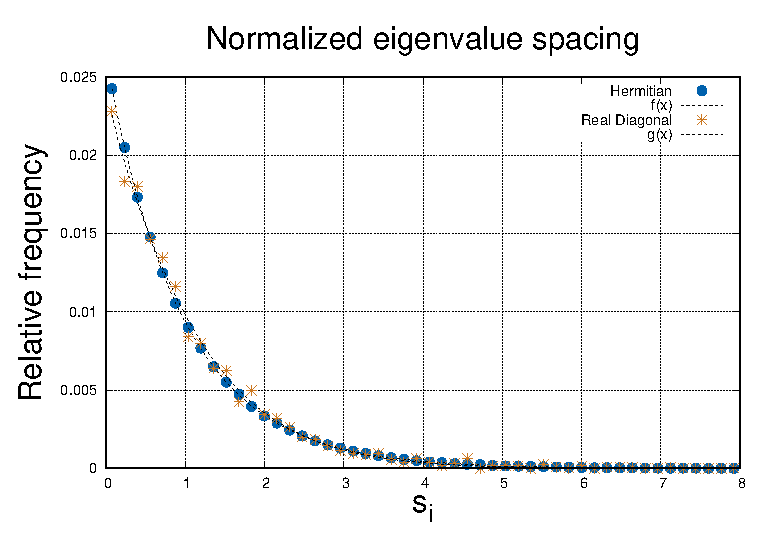
\includegraphics[width=\textwidth]{Hist_2000_0450.eps}
\caption{Normalized eigenvalue spacings from random Hermitian matrices (blue) and from random real diagonal matrices (orange).}
\label{fig:histofit}
\end{figure}

\begin{table}[h]
\centering
\caption{Fit results for Hermitian (first row) and real diagonal (second row) matrices.}
\label{tab:mu_lit}
\begin{minipage}{16cm}
\[
\begin{array}{cccccc}
%               la tabella inizia qui
\toprule    

 &\bm{a} & \bm{\alpha} & \bm{b} & \bm{\beta} & \bm{\chi^2}/\textbf{d.o.f.}\\
\midrule
f(x) & 0.0263 \pm 0.0002 &   -0.001\pm 0.003 & 1.033 \pm 0.008 & 0.987 \pm 0.002 &1.6\times 10^{-8}\\
g(x) & 0.021\pm  0.002  &   -0.04 \pm 0.04  & 0.8 \pm 0.1 &  1.2 \pm 0.1 \pm 0.005 & 3\times10^{-4}\\

\bottomrule                                                 
%               la tabella finisce qui
\end{array}
\]
\end{minipage}
\end{table}
As a conclusion we can observe that some parameters of the two distributions are not compatible and therefore we cannot state that they are the same.
Nonetheless the similarity between the two is remarkable and it is a clear sign of correlation, which might be confirmed by more specific analysis.


\end{document}
